\documentclass[twocolumn,preprintnumbers,superscriptaddress]{revtex4-2}
\usepackage{amsmath}
\usepackage{amssymb}
\usepackage{graphicx}
\usepackage{hyperref}
\usepackage{physics}
\usepackage{xcolor}
\usepackage{xspace,slashed}
\usepackage{qcircuit}
\usepackage{multirow}
\usepackage[utf8]{inputenc}
\usepackage{subfigure}

\usepackage{array}

\begin{document}

\title{
  Generating LHC events with a quantum generative model
 }

\preprint{CERN-TH-xx, TIF-UNIMI-2021-xx}

\newcommand{\CERNaff}{Theoretical Physics Department, CERN, CH-1211
  Geneva 23, Switzerland.}

\newcommand{\tii}{Quantum Research Centre, Technology Innovation Institute, Abu Dhabi, UAE}

\newcommand{\bern}{Albert Einstein Center, CH-3012 Bern, Switzerland}

\newcommand{\UB}{Departament de F\'isica Qu\`antica i Astrof\'isica and Institut de Ci\`encies del Cosmos (ICCUB), Universitat de Barcelona, Barcelona, Spain.}

\newcommand{\MIaff}{TIF Lab, Dipartimento di Fisica, Universit\`a degli Studi di
  Milano and INFN Sezione di Milano, Milan, Italy.}

\author{Carlos Bravo-Prieto}
\affiliation{\tii}
\affiliation{\UB}

\author{Julien Baglio}
\affiliation{\CERNaff}

\author{Marco Cè}
\affiliation{\CERNaff}

\author{Anthony Francis}
\affiliation{\bern}

\author{Dorota Grabowska}
\affiliation{\CERNaff}

\author{Stefano Carrazza}
\affiliation{\MIaff}
\affiliation{\CERNaff}
\affiliation{\tii}


\begin{abstract}
    We present a first attempt to design a quantum circuit for the generation of
    Monte Carlo simulated events using quantum generative models, in the context
    of high energy physics (HEP). The growing interest in quantum computing and
    the recent developments of new algorithms and quantum hardware devices
    motivates the study of methodologies applied to HEP. In this work we
    identify architectures of variational quantum circuits suitable for
    designing a generative model for Monte Carlo event generation. We show
    experiments on artificial data generated from known underlying
    distributions. Finally, we train a quantum GAN using Monte Carlo events and
    benchmark the performance in terms of quality and performance.
\end{abstract}

\maketitle

\section{Introduction}

Quantum computing is a new computation paradigm that exploits the laws of
quantum mechanics to provide new strategies for addressing problems that are
nowadays considered to be difficult. The first quantum algorithms showing any
advantage over their classical counterparts date from the 1990s, being Shor's
algorithm for integer factorization and Grover's search the most prominent
ones~\cite{shor,grover}. During the last decade, we have witnessed an
impressively fast development of quantum computing, both for theoretical work
and hardware implementation perspectives. Nevertheless, currently existing
quantum devices are not powerful enough to run competitive quantum algorithms,
with respect to the state of the art of the classical ones.

Recent achievements such as {\sl quantum supremacy}~\cite{supremacy} have
introduced the so-called Noisy Intermediate-Scale Quantum (NISQ)
stage~\cite{nisq}. NISQ devices suffer from errors due to decoherence, noisy
gates and erratic read-out measurements, and thus, its performance is limited.
However, even at this early stage, quantum technologies may provide useful tools
for a broad range of applications. On the one hand, some standard fully
determined algorithms are well suited for NISQ
processors~\cite{cerveralierta:2018ising,suba:2019spectroscopy,bravyi:2018shallow,Bravyi:2020noisyshallow,ramoscalderer:2020unary}.
In particular, there also exist some examples of quantum algorithms designed to
address some problems in high energy physics
(HEP)~\cite{Perez-Salinas:2020nem,hep_amplitudes-bepari2020, hep_simulation-bauer2019,
hep_gluon-alexandru2019, hep_parton-lamm2020}. On the other hand, the approach
usually taken to harness the computational power of these imperfect machines is
based on hybrid methods combining quantum and classical resources. For example,
variational algorithms can be created whose purpose is to optimize some quantity
encoding a solution for a specific problem. Among the great variety of quantum
variational algorithms it is possible to find examples in quantum
chemistry~\cite{peruzzo:2014vqe,higgott:2019vqe,aspuru:2005molecular,hempel:2018chemistry,jones:2019vqe},
quantum
simulation~\cite{li:2017simulation,kokail:2019simulation,cirstoiu:2020simulation},
combinatorial optimization~\cite{farhi:2014qoao}, solving linear systems of
equations~\cite{bravoprieto:2020linear,xu:2019linear,huang:2019linear} and state
diagonalization
~\cite{LaRose:2019diagonalization,BravoPrieto:2020diagonalization}. Some of
these examples are already characterized as Quantum Machine Learning (QML)
applications, based on variational~\cite{perezsalinas:2020reuploading,
mitarai:2018circuit,Zhu:2019circuit,Schuld:2020circuit,lloyd:2020embeddings} and
non-variational~\cite{liu:2020svm,Rebentrost:2014svm,lloyd:2013ml} approaches.
Furthermore, QML is a field that is expected to surpass the current performance
and ubiquity of classical Machine Learning (ML) when the current limitations of
quantum devices will be overcome.

The QML approach to quantum computing is an interesting research topic which can
be adapted and tested on research problems already addressed by ML techniques.
Motivated by this idea, we propose to investigate the possibility to use quantum
computing for the generation of Monte Carlo events through quantum generative
adversarial circuits.

There are different reasons for attempting a qMCGAN determination. First,
quantum computing is expected to have a reduced energy consumption when compared
to an equivalent classical computer, and thus, we may expect saving power and
reducing its environmental impact. Secondly, as we show in this work, the number
of parameters needed to obtain an acceptable generator is in average lower with
quantum models in comparison to modern GAN models. Furthermore, the qMCGAN
approach may take advantage from quantum entanglement, since the potential
outstanding power of quantum computing emerges from there. Finally, quantum
hardware may bring performance improvements in terms of running time for this
model when compared to the standard ML approach since the number of operations
needed to obtain an acceptable solution is lower and the model has an exact
hardware representation. On the other hand, we consider the qMCGAN model
presented in this work as proof-of-concept for future implementations, given
that the performance of quantum simulation on classical hardware and the
stability of real quantum device measurements are not competitive yet.

The paper is structured as follows. Sec.~\ref{sec:implementation} we identify
the best qMCGAN architecture. In Sec.~\ref{sec:validation} we validate the
qMCGAN model using toy data. In Sec.~\ref{sec:lhc} we train the qMCGAN generator
on simulated LHC events. Finally, in Sec.~\ref{sec:conclusion} we present our
conclusion and future development directions.

\section{Implementation}
\label{sec:implementation}

\begin{enumerate}
  \item Talk about model definition
  \item Talk about training procedure
  \item Talk about circuit deployment changes between simulation and IBM
\end{enumerate}

\begin{figure*}
  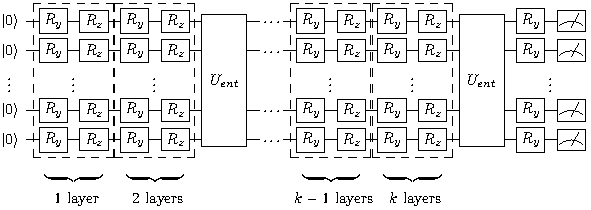
\includegraphics[width=0.8\textwidth]{plots/ansatz1.pdf}
  \caption{\label{fig:circuit}Ansatz 1 for the quantum generator.}
\end{figure*}

\begin{figure*}
  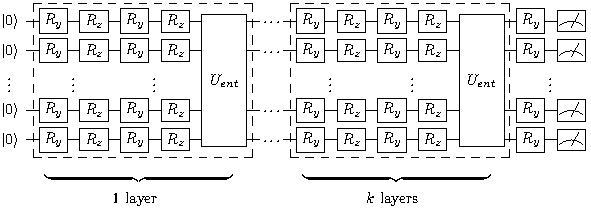
\includegraphics[width=0.8\textwidth]{plots/ansatz2.pdf}
  \caption{\label{fig:circuit}Ansatz 2 for the quantum generator.}
\end{figure*}

\section{Validation}
\label{sec:validation}

\begin{enumerate}
  \item Show 1D example (histograms + KL) for different (layers, latent) dim.
  \item Show 2D example (histograms + KL) for different (layers, latent) dim.
  \item Show 3D gaussian example for different (layers, latent) dim.
\end{enumerate}

\begin{figure}
  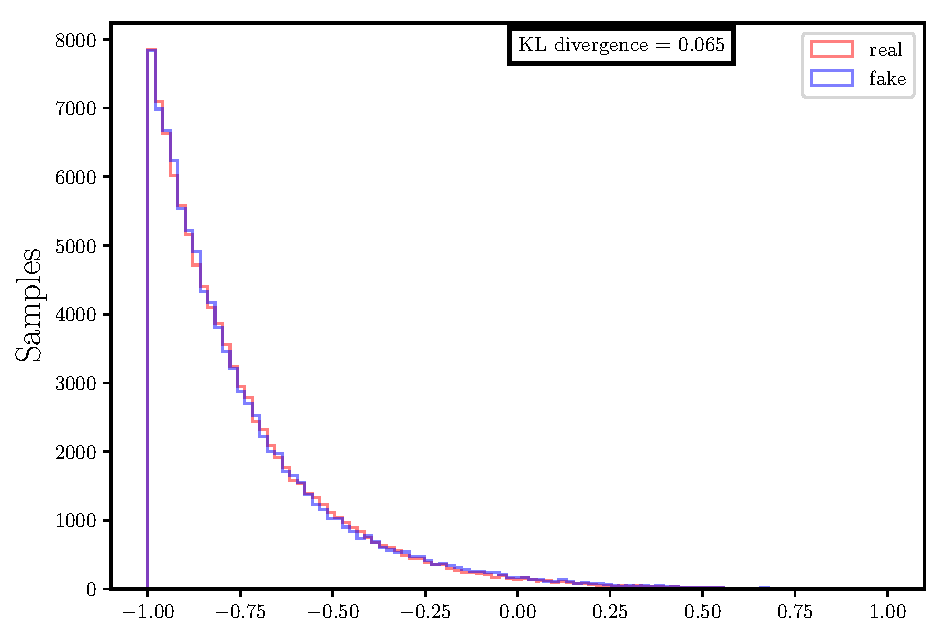
\includegraphics[width=0.45\textwidth]{plots/1Dgamma/1-distribution_100000_100_1_3_2_10000_128_0.5.pdf}\\
  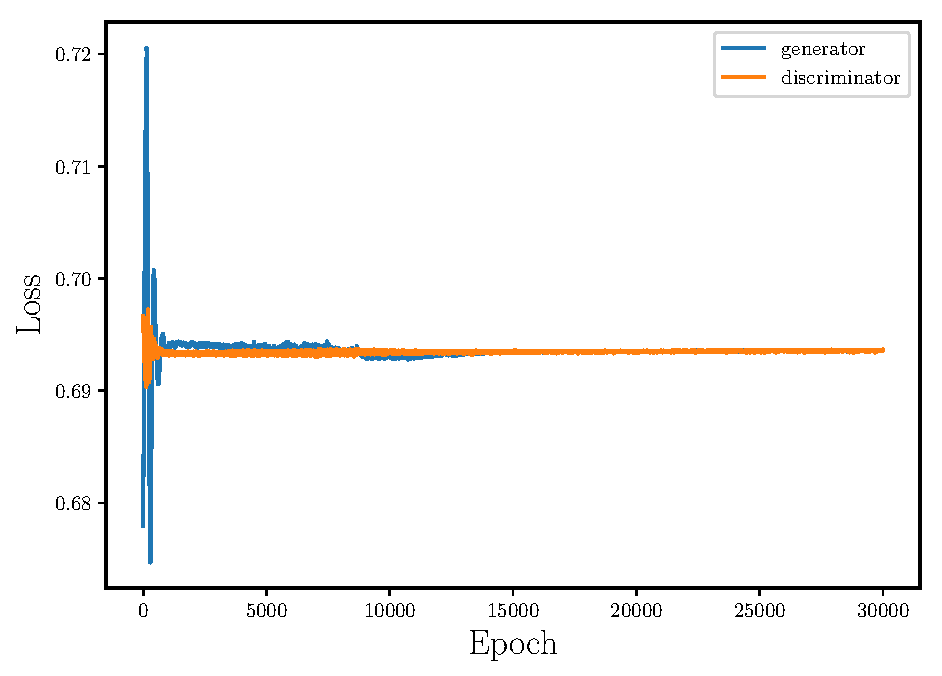
\includegraphics[width=0.45\textwidth]{plots/1Dgamma/loss_100000_100_1_3_2_10000_128_0.5.pdf}
  \caption{Example of 1D gamma distribution.}
\end{figure}

\begin{figure*}
  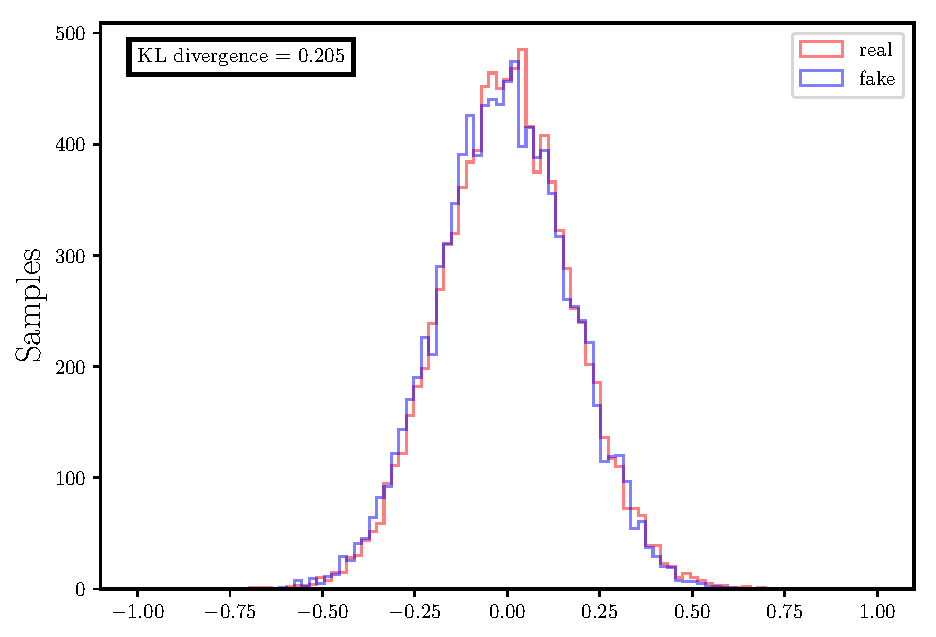
\includegraphics[width=0.25\textwidth]{plots/3Dgaussian_posdef/1-distribution_10000_100_3_5_2_10000_128_0.5.pdf}%
  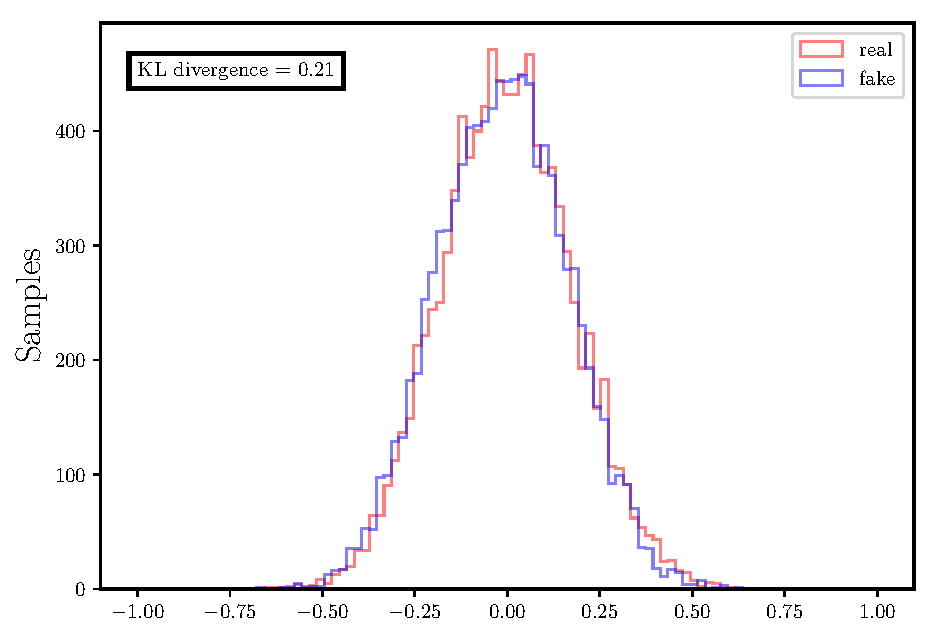
\includegraphics[width=0.25\textwidth]{plots/3Dgaussian_posdef/2-distribution_10000_100_3_5_2_10000_128_0.5.pdf}%
  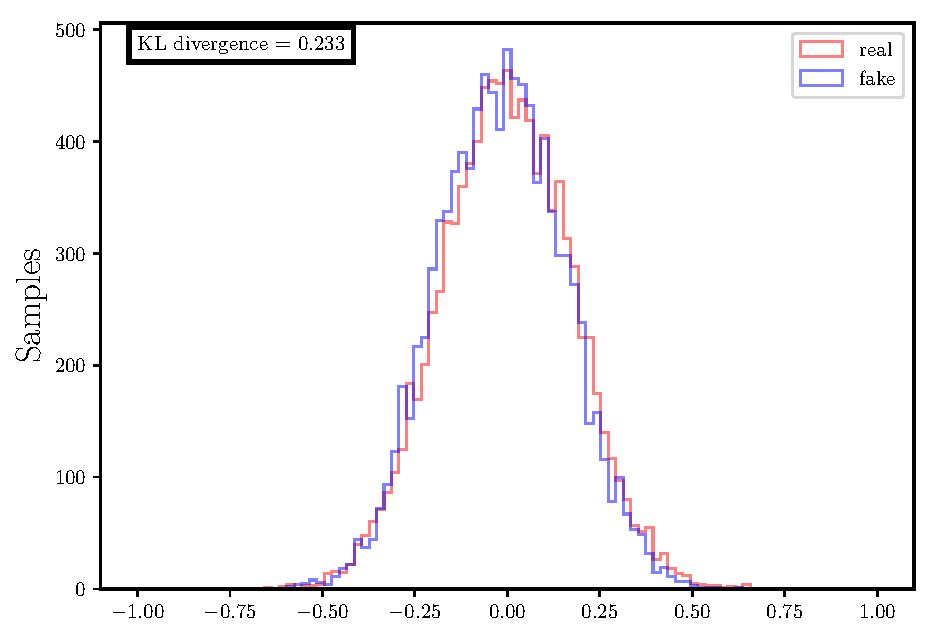
\includegraphics[width=0.25\textwidth]{plots/3Dgaussian_posdef/3-distribution_10000_100_3_5_2_10000_128_0.5.pdf}

  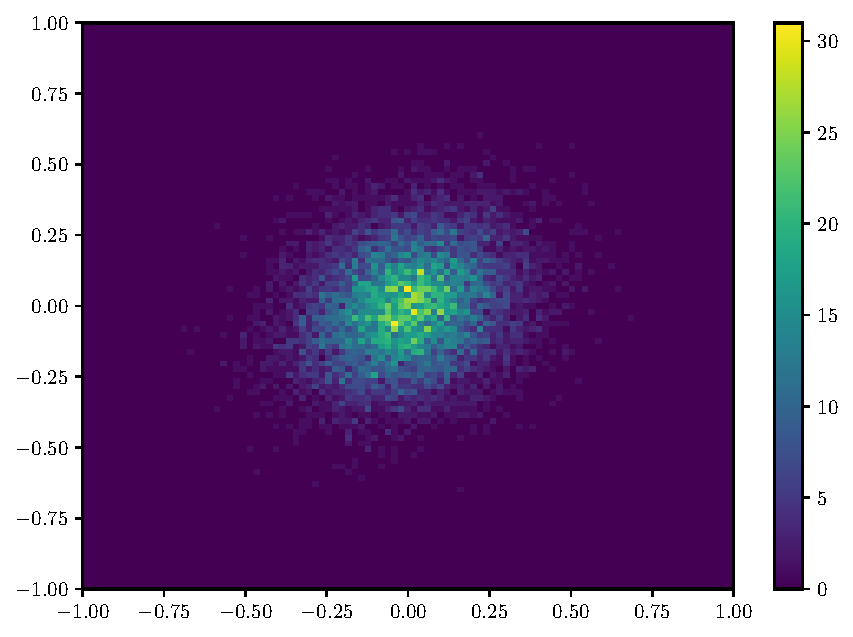
\includegraphics[width=0.25\textwidth]{plots/3Dgaussian_posdef/1-2_REAL_10000_100.pdf}%
  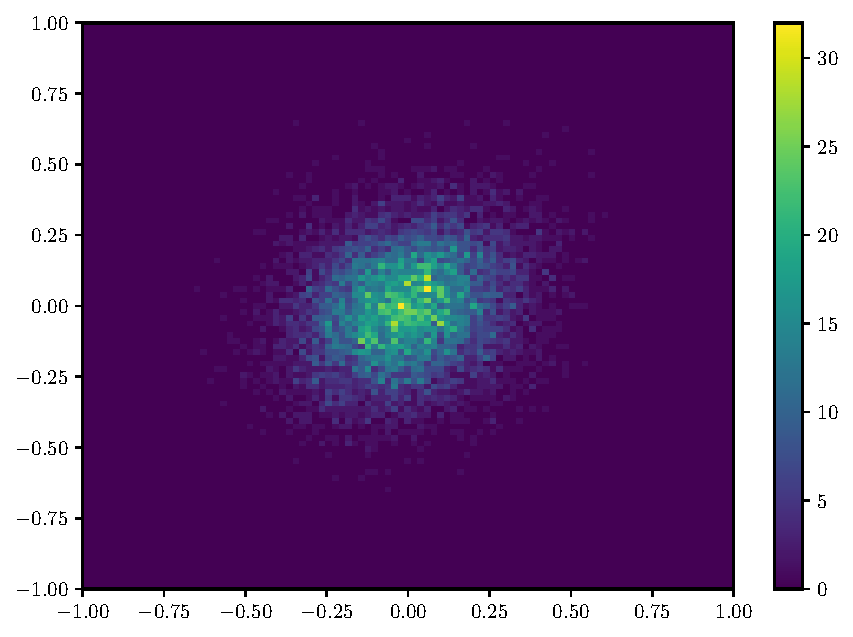
\includegraphics[width=0.25\textwidth]{plots/3Dgaussian_posdef/2-3_REAL_10000_100.pdf}%
  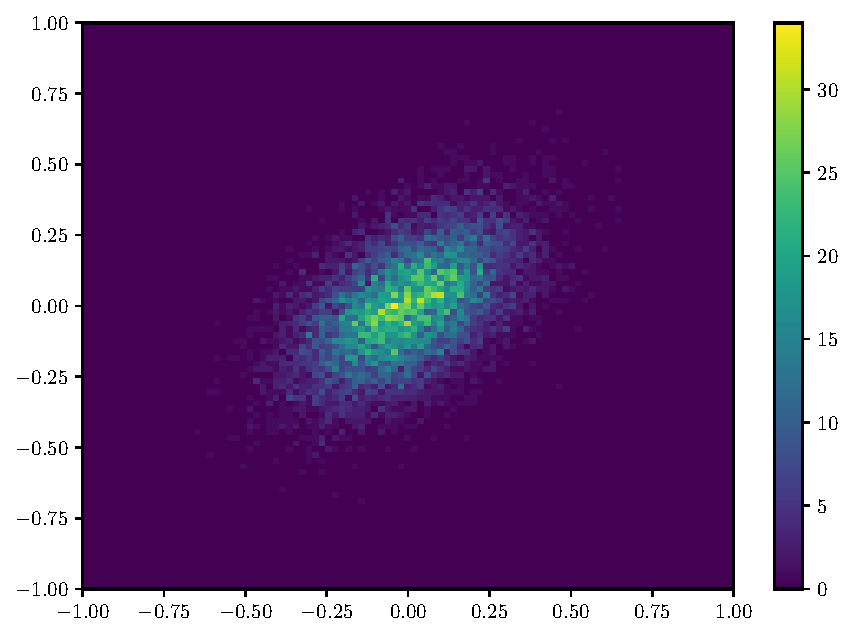
\includegraphics[width=0.25\textwidth]{plots/3Dgaussian_posdef/3-1_REAL_10000_100.pdf}

  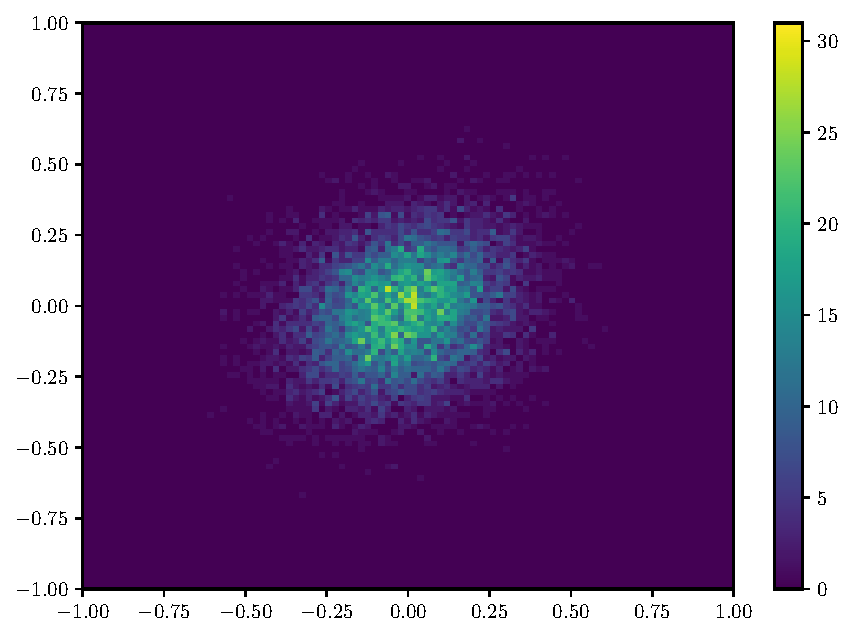
\includegraphics[width=0.25\textwidth]{plots/3Dgaussian_posdef/1-2_FAKE_10000_100_3_5_2_10000_128_0.5.pdf}%
  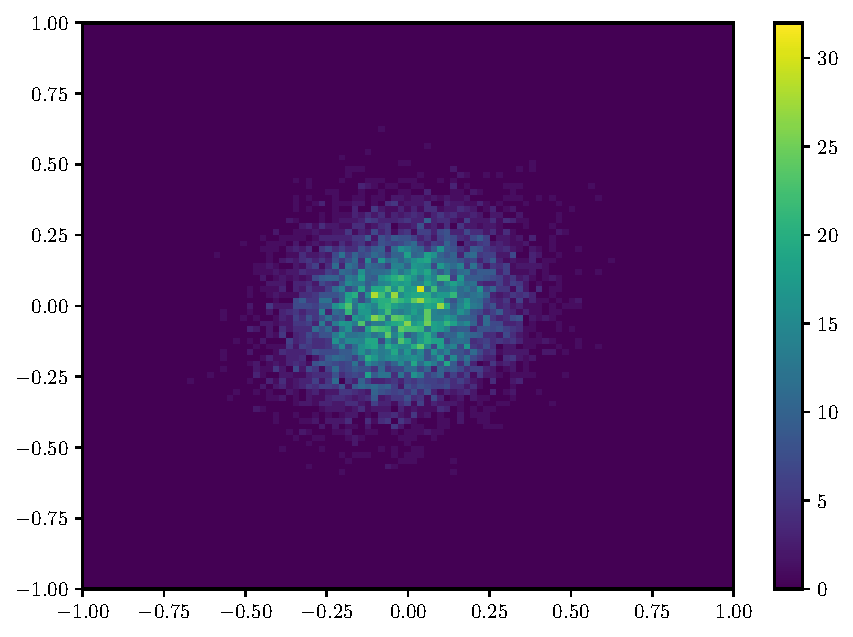
\includegraphics[width=0.25\textwidth]{plots/3Dgaussian_posdef/2-3_FAKE_10000_100_3_5_2_10000_128_0.5.pdf}%
  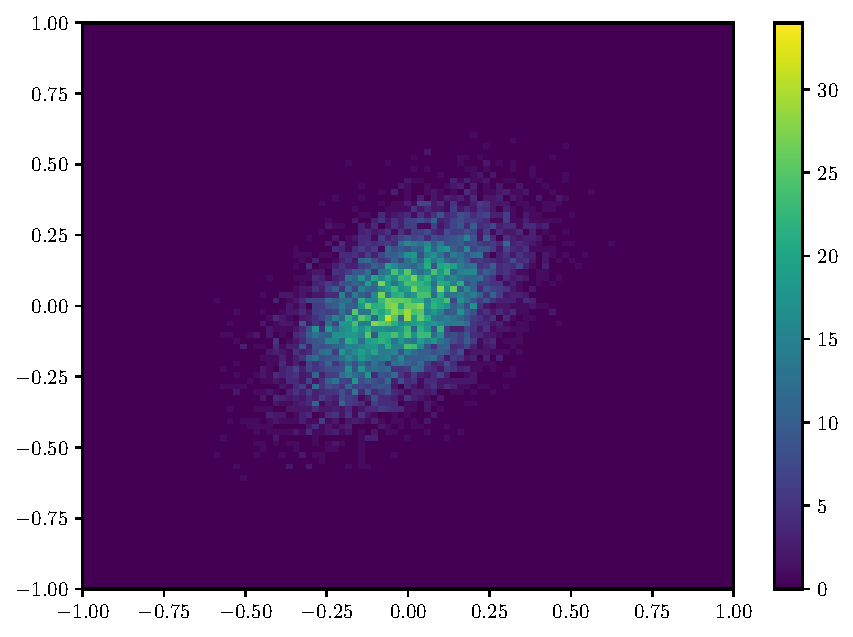
\includegraphics[width=0.25\textwidth]{plots/3Dgaussian_posdef/3-1_FAKE_10000_100_3_5_2_10000_128_0.5.pdf}
  \caption{\label{fig:3dgauss}Example of samples generated for a 3D correlated
  multivariate normal distribution using a QGAN generator model.}
\end{figure*}

\begin{figure*}
  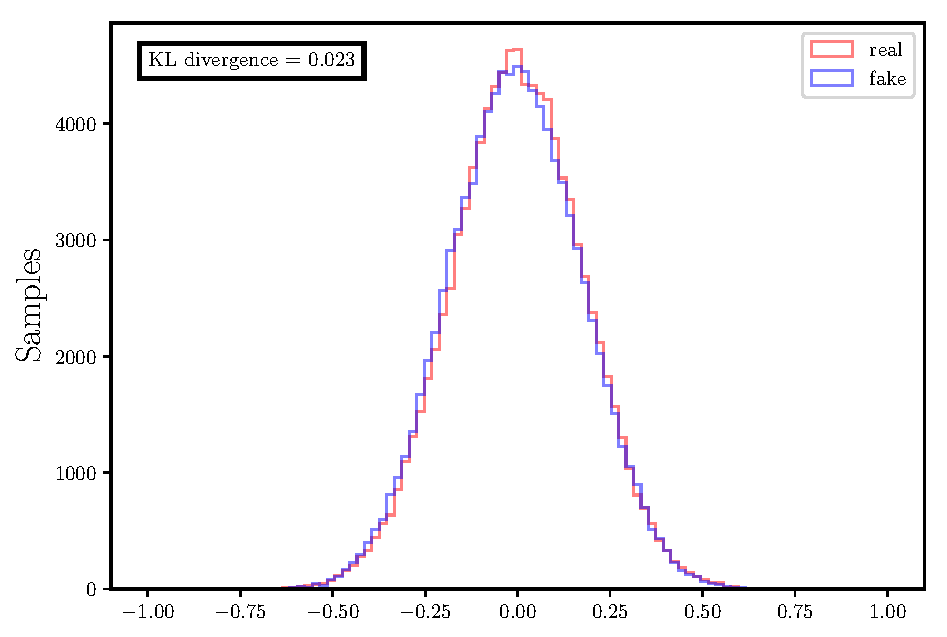
\includegraphics[width=0.25\textwidth]{plots/3Dgaussian_posdef/1-distribution_100000_100_3_5_2_10000_128_0.5.pdf}%
  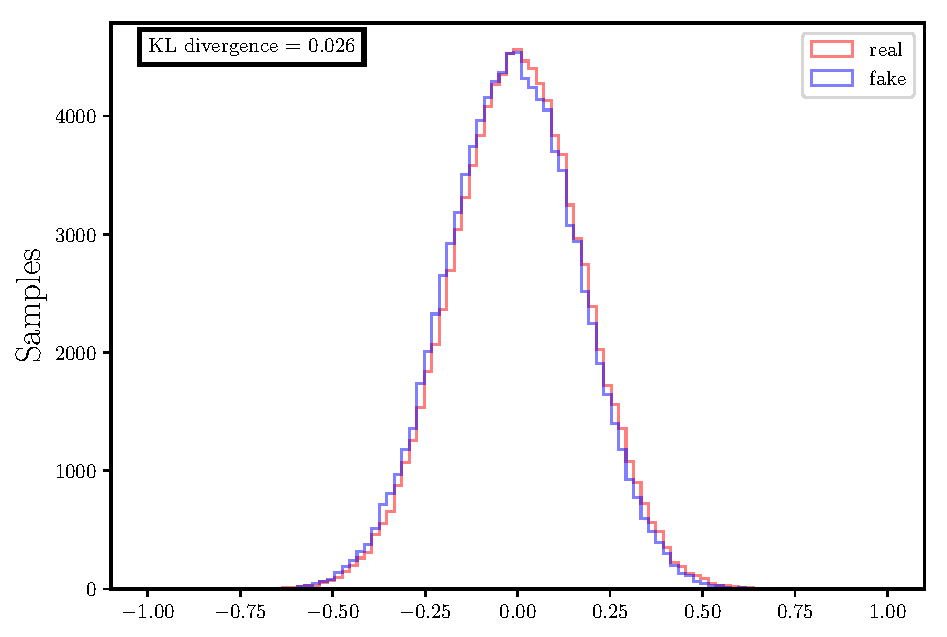
\includegraphics[width=0.25\textwidth]{plots/3Dgaussian_posdef/2-distribution_100000_100_3_5_2_10000_128_0.5.pdf}%
  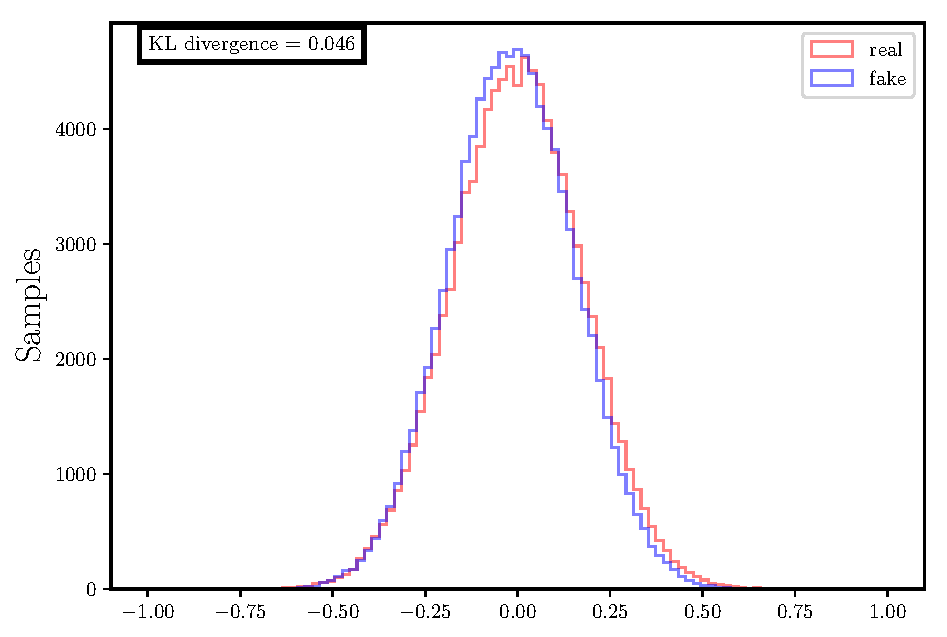
\includegraphics[width=0.25\textwidth]{plots/3Dgaussian_posdef/3-distribution_100000_100_3_5_2_10000_128_0.5.pdf}

  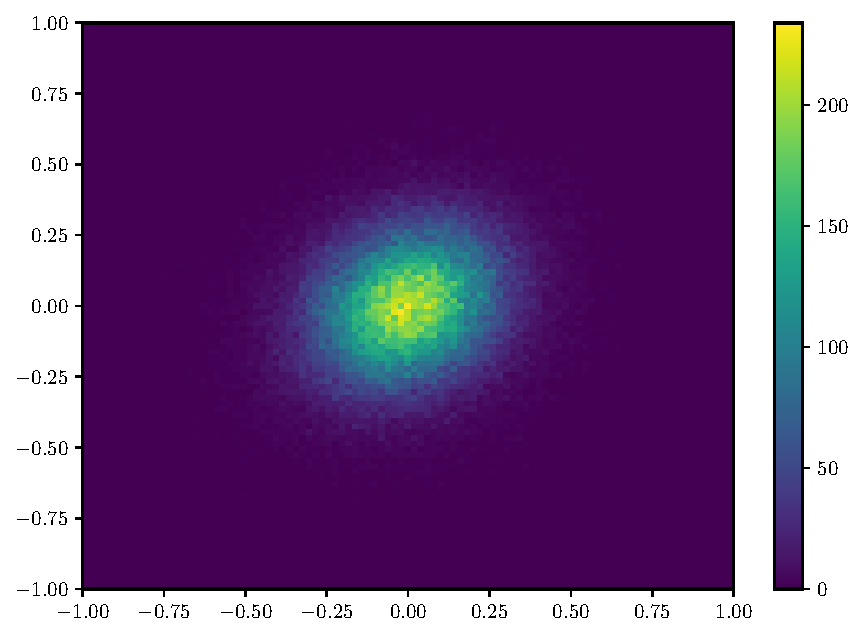
\includegraphics[width=0.25\textwidth]{plots/3Dgaussian_posdef/1-2_REAL_100000_100.pdf}%
  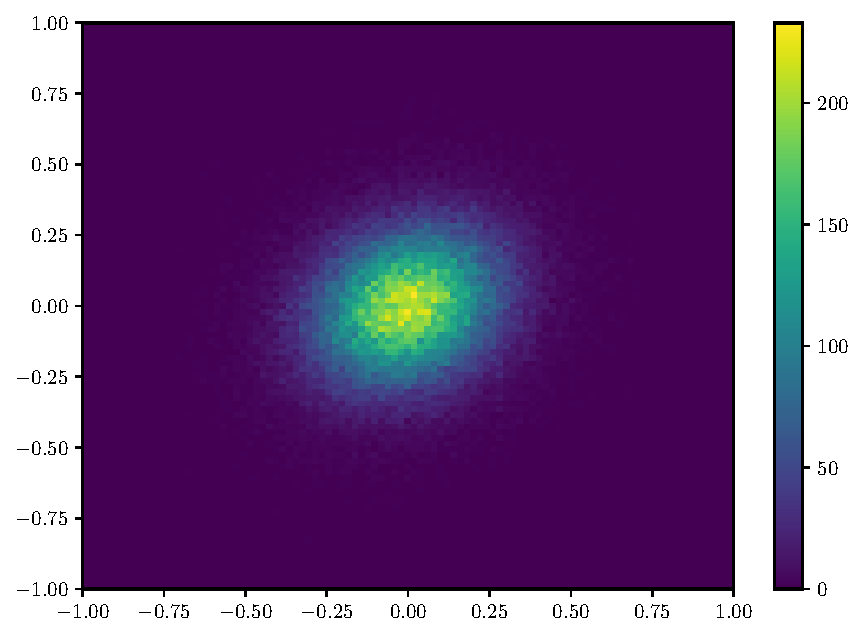
\includegraphics[width=0.25\textwidth]{plots/3Dgaussian_posdef/2-3_REAL_100000_100.pdf}%
  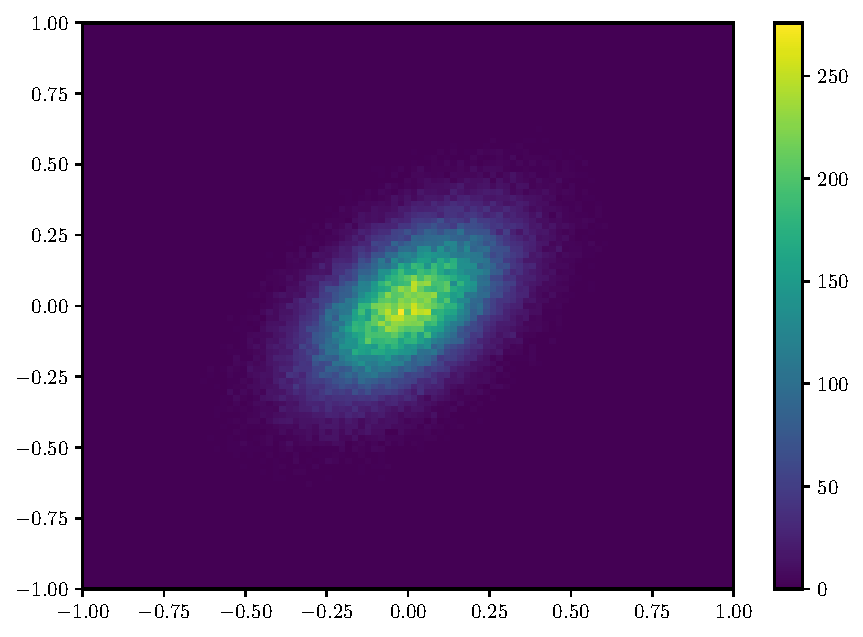
\includegraphics[width=0.25\textwidth]{plots/3Dgaussian_posdef/3-1_REAL_100000_100.pdf}

  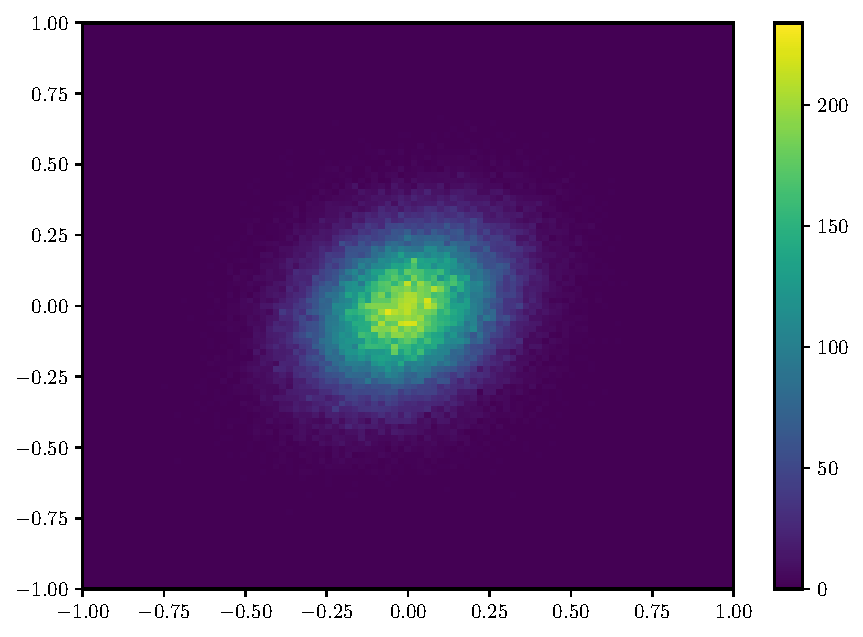
\includegraphics[width=0.25\textwidth]{plots/3Dgaussian_posdef/1-2_FAKE_100000_100_3_5_2_10000_128_0.5.pdf}%
  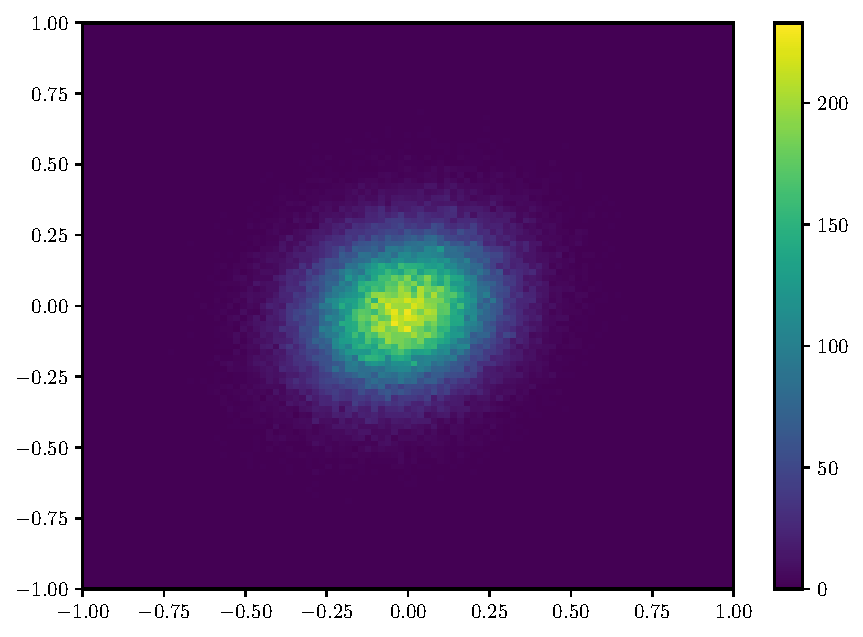
\includegraphics[width=0.25\textwidth]{plots/3Dgaussian_posdef/2-3_FAKE_100000_100_3_5_2_10000_128_0.5.pdf}%
  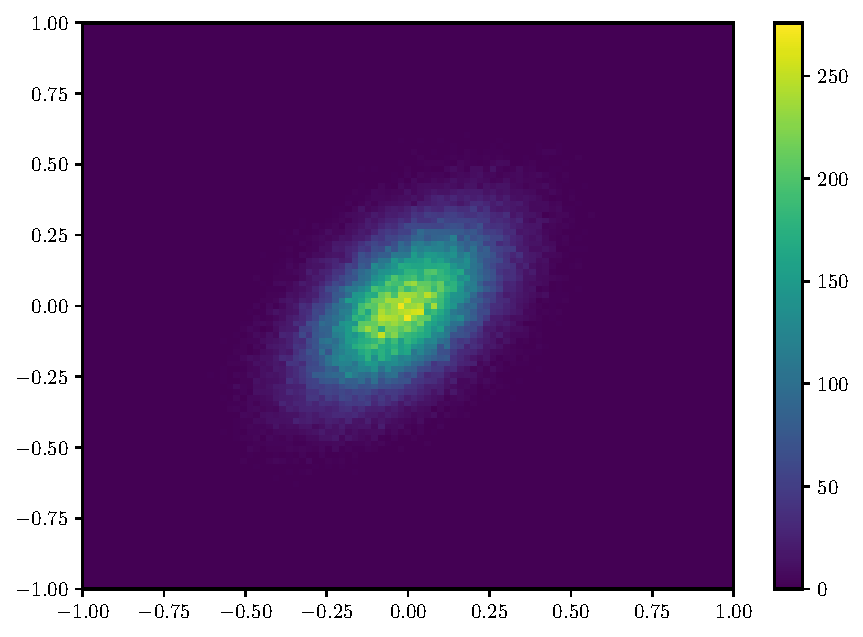
\includegraphics[width=0.25\textwidth]{plots/3Dgaussian_posdef/3-1_FAKE_100000_100_3_5_2_10000_128_0.5.pdf}
  \caption{\label{fig:3dgauss}Example of samples generated for a 3D correlated
  multivariate normal distribution using a QGAN generator model.}
\end{figure*}

\section{Generating LHC events}
\label{sec:lhc}

\begin{enumerate}
  \item Show ttbar and WW results, histograms, KL, correlations, etc.
  \item Provide hints concerning data augmentation.
  \item Show experimental results obtained with quantum hardware, identify the
  best features, pro and cons of different hardware.
\end{enumerate}

\begin{figure*}
  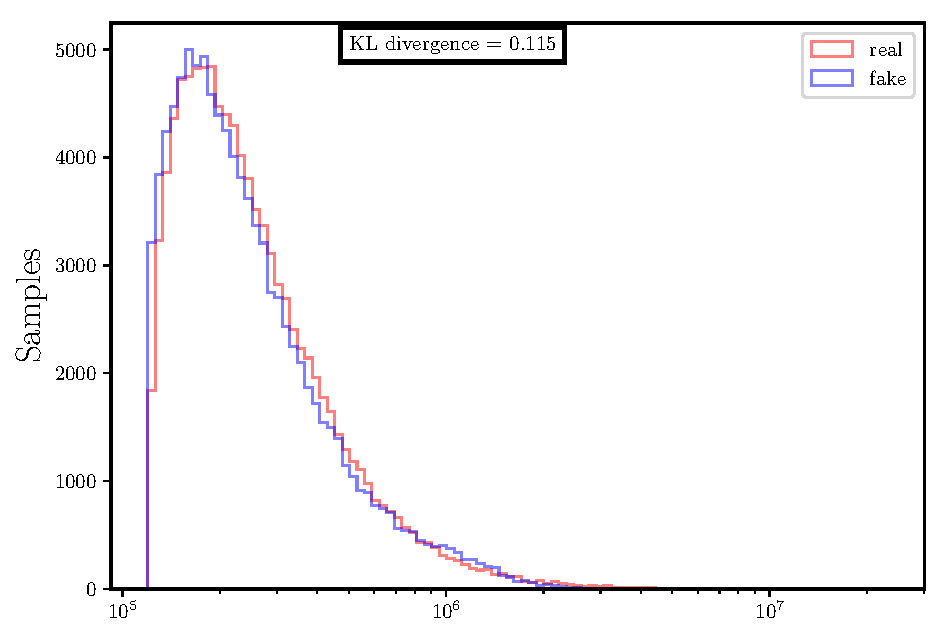
\includegraphics[width=0.25\textwidth]{plots/LHCttbar/s-distribution_100000_100_3_5_4_10000_128_0.5.pdf}%
  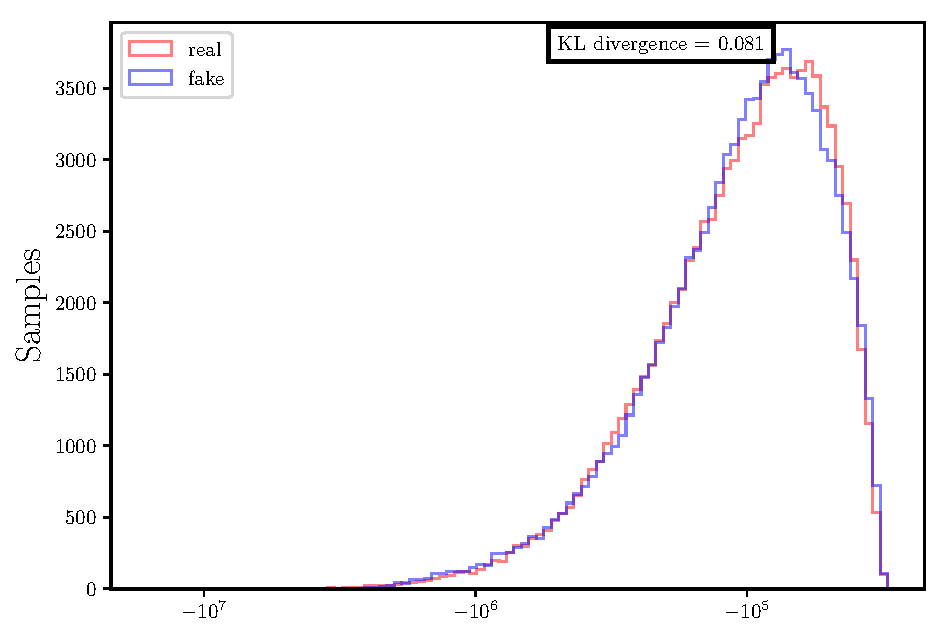
\includegraphics[width=0.25\textwidth]{plots/LHCttbar/t-distribution_100000_100_3_5_4_10000_128_0.5.pdf}%
  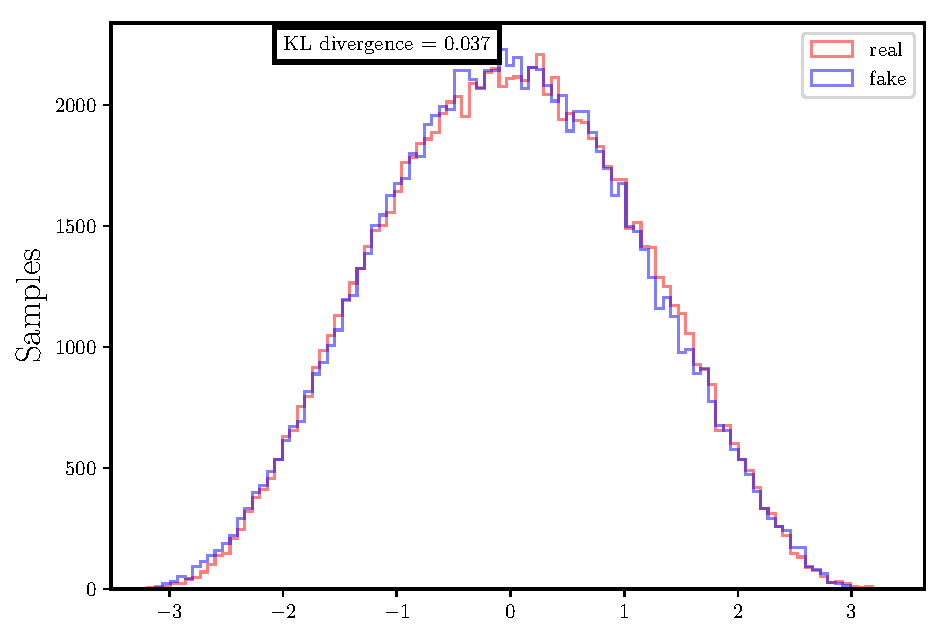
\includegraphics[width=0.25\textwidth]{plots/LHCttbar/y-distribution_100000_100_3_5_4_10000_128_0.5.pdf}

  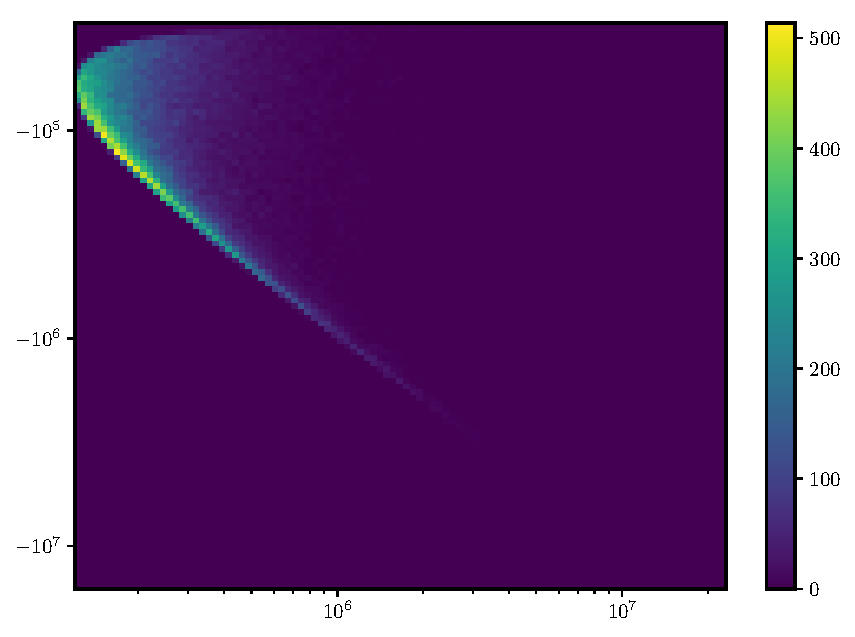
\includegraphics[width=0.25\textwidth]{plots/LHCttbar/s-t_REAL_100000_100.pdf}%
  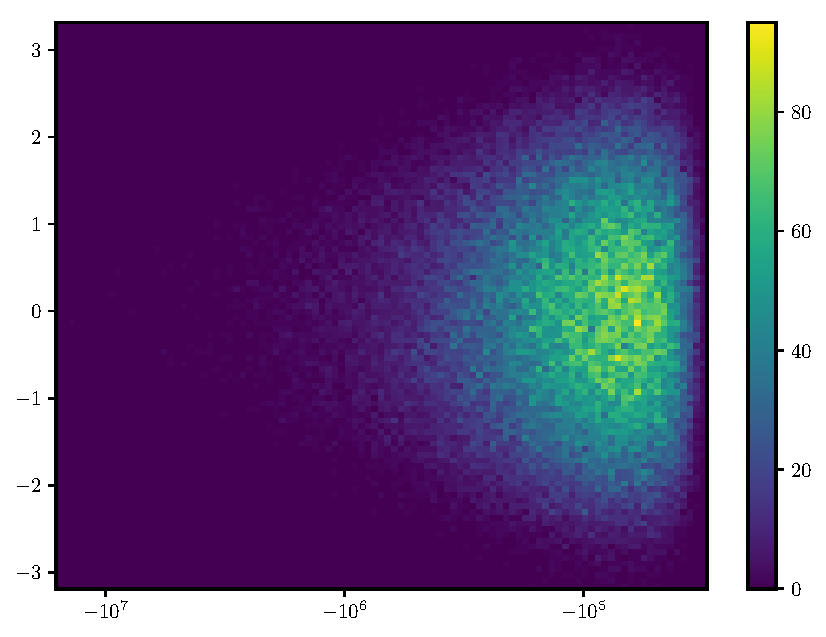
\includegraphics[width=0.25\textwidth]{plots/LHCttbar/t-y_REAL_100000_100.pdf}%
  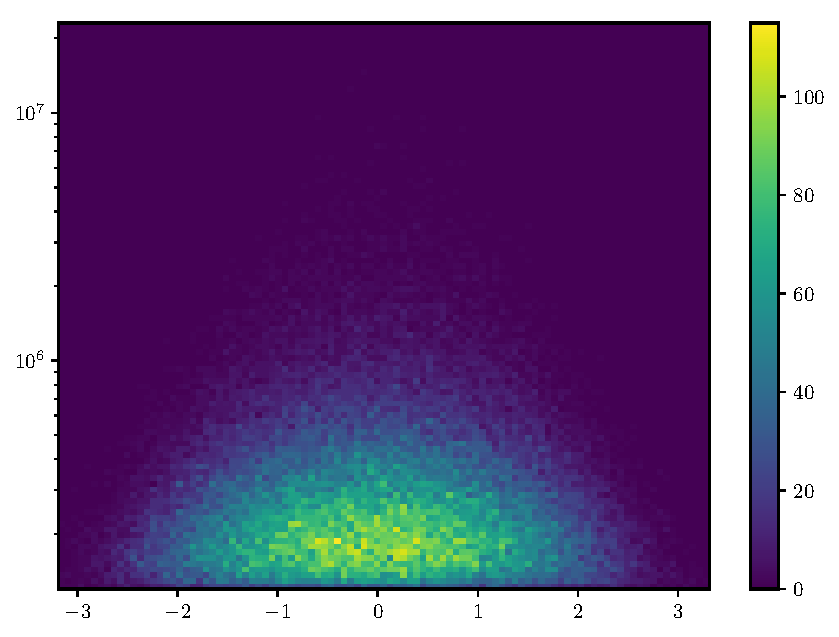
\includegraphics[width=0.25\textwidth]{plots/LHCttbar/y-s_REAL_100000_100.pdf}

  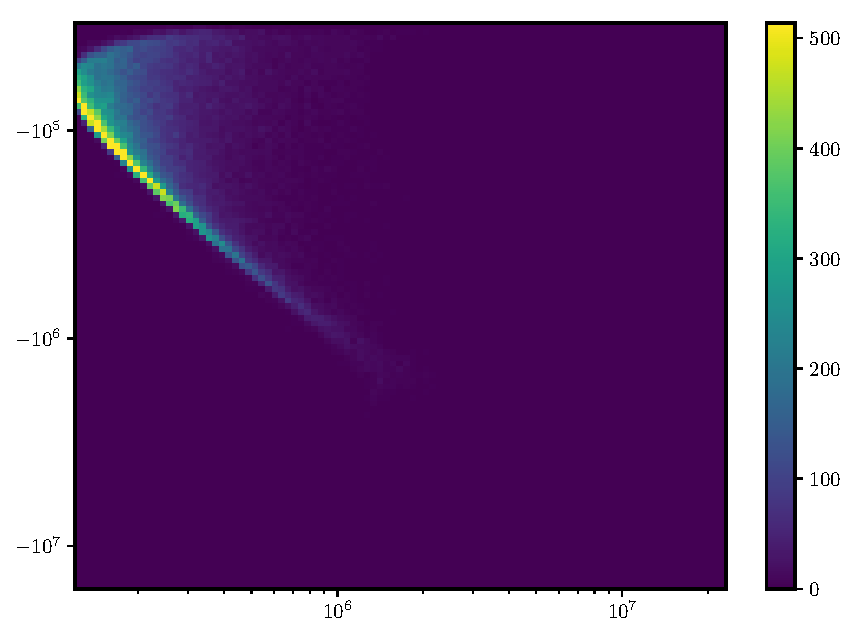
\includegraphics[width=0.25\textwidth]{plots/LHCttbar/s-t_FAKE_100000_100_3_5_4_10000_128_0.5.pdf}%
  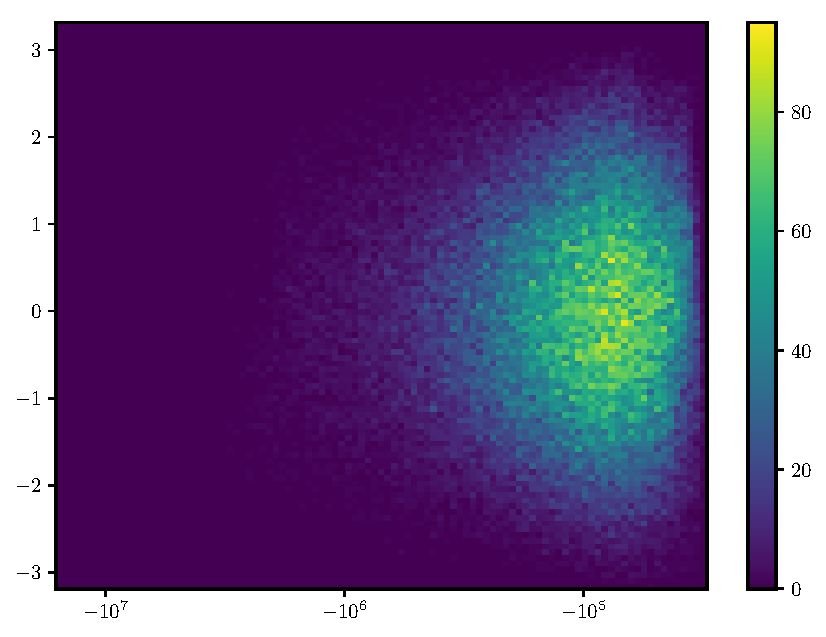
\includegraphics[width=0.25\textwidth]{plots/LHCttbar/t-y_FAKE_100000_100_3_5_4_10000_128_0.5.pdf}%
  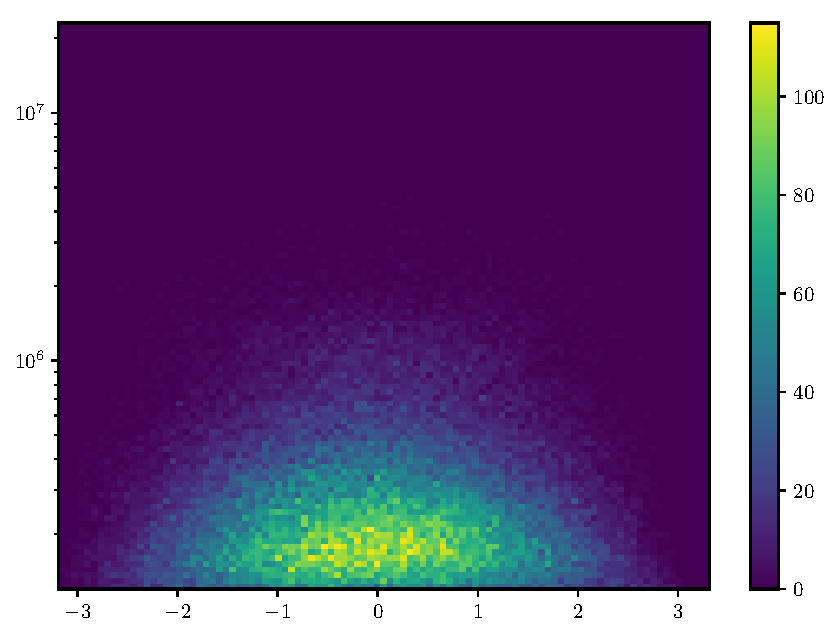
\includegraphics[width=0.25\textwidth]{plots/LHCttbar/y-s_FAKE_100000_100_3_5_4_10000_128_0.5.pdf}

  \caption{\label{fig:3dgauss}Example of samples generated for a $t\bar{t}$
  production using a QGAN generator model.}
\end{figure*}

\section{Sampling from real quantum hardware}

{\color{red}[SC: Julien and Marco please summarize the experimental setup]}

\begin{figure*}
  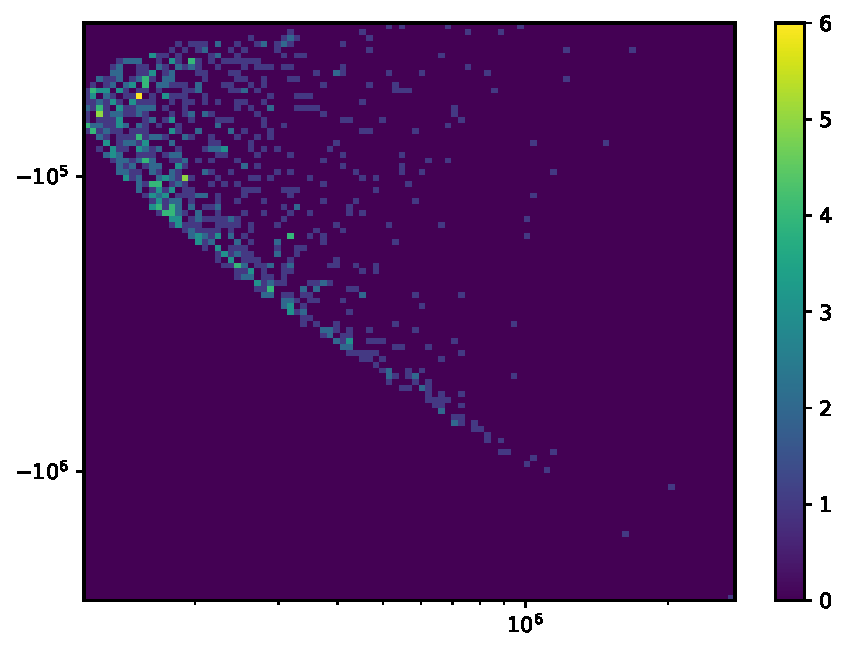
\includegraphics[width=0.25\textwidth]{plots/hardware_1k/ibm_lagos/s-t_REAL_1000_100.pdf}%
  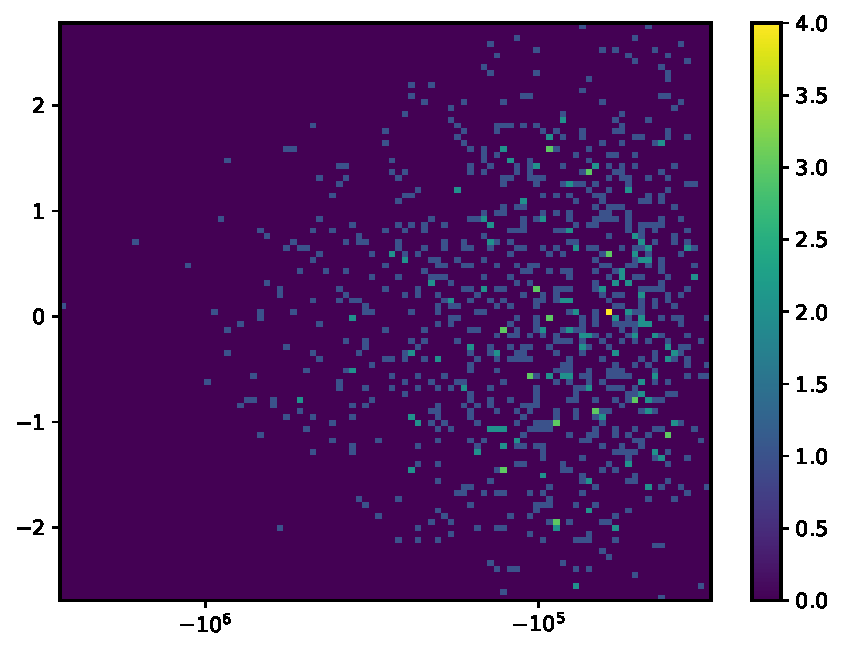
\includegraphics[width=0.25\textwidth]{plots/hardware_1k/ibm_lagos/t-y_REAL_1000_100.pdf}%
  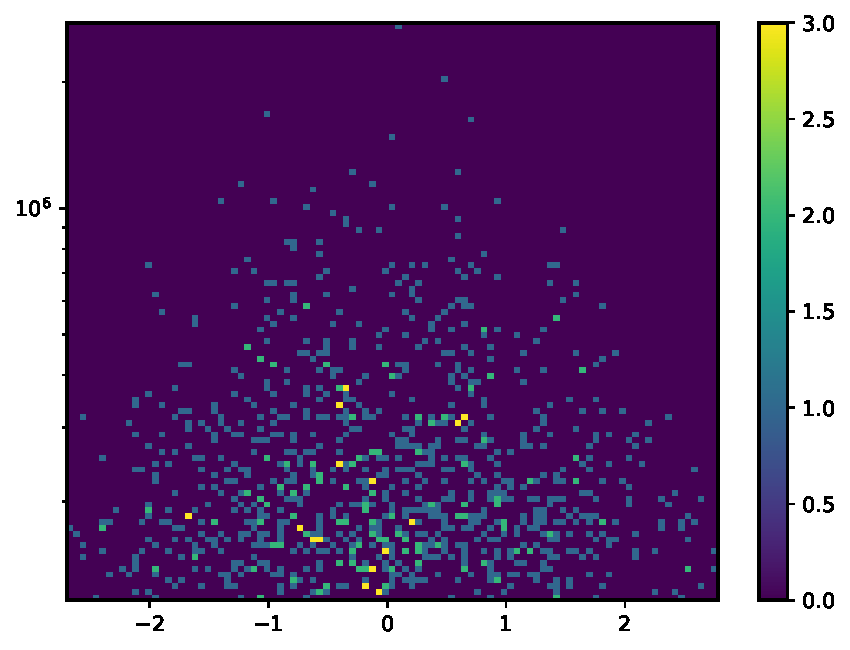
\includegraphics[width=0.25\textwidth]{plots/hardware_1k/ibm_lagos/y-s_REAL_1000_100.pdf}

  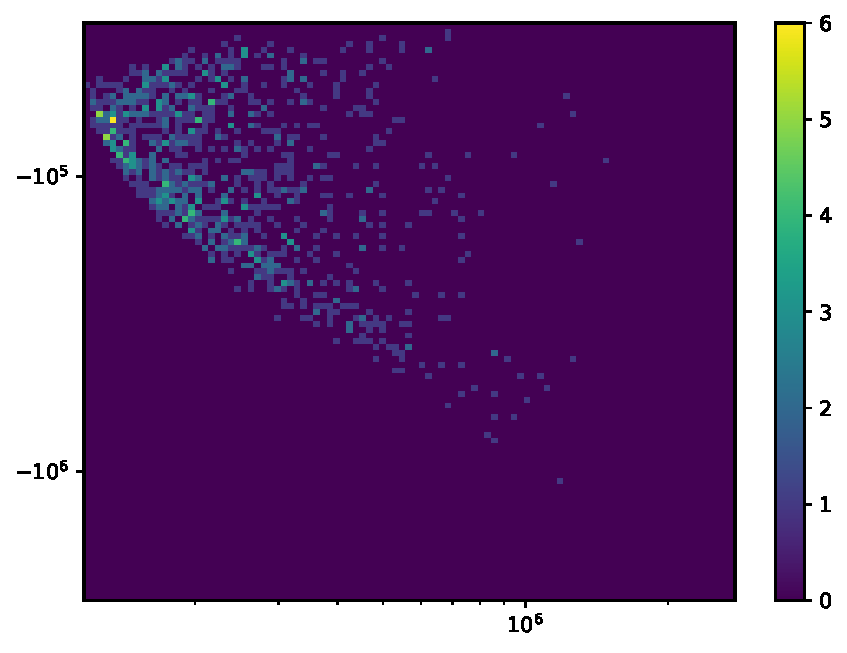
\includegraphics[width=0.25\textwidth]{plots/hardware_1k/ibm_lagos/s-t_FAKE_1000_100_3_5_2_10000_128_0.5_1024.pdf}%
  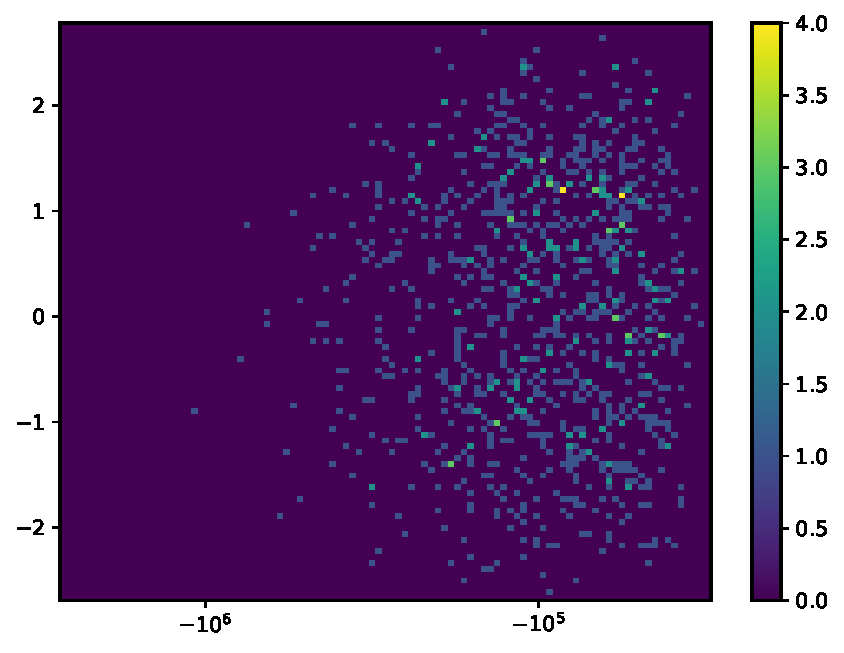
\includegraphics[width=0.25\textwidth]{plots/hardware_1k/ibm_lagos/t-y_FAKE_1000_100_3_5_2_10000_128_0.5_1024.pdf}%
  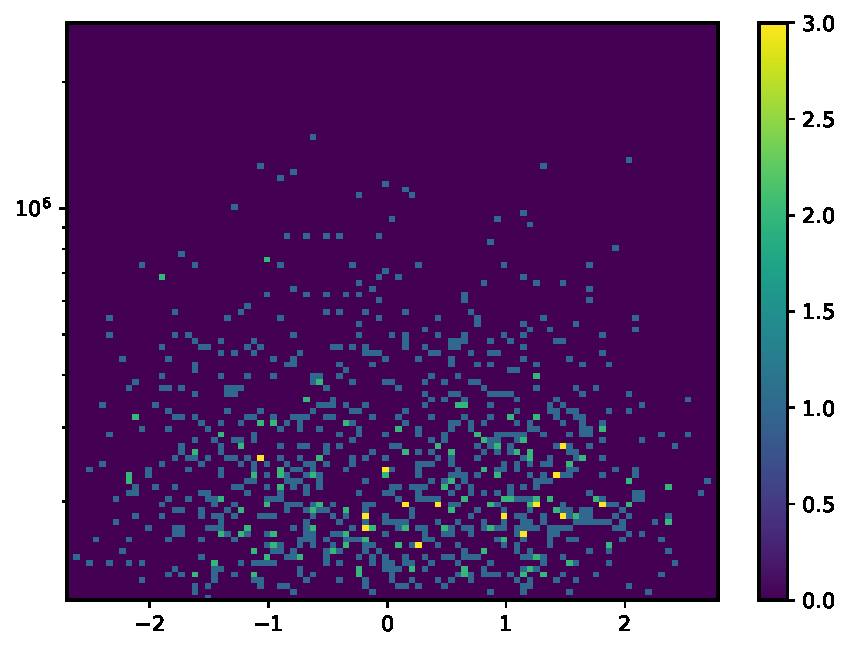
\includegraphics[width=0.25\textwidth]{plots/hardware_1k/ibm_lagos/y-s_FAKE_1000_100_3_5_2_10000_128_0.5_1024.pdf}

  \caption{\label{fig:3dgauss}Example of samples generated for a $t\bar{t}$
  production using a QGAN generator model on IBM Lagos.}
\end{figure*}

\begin{figure*}
  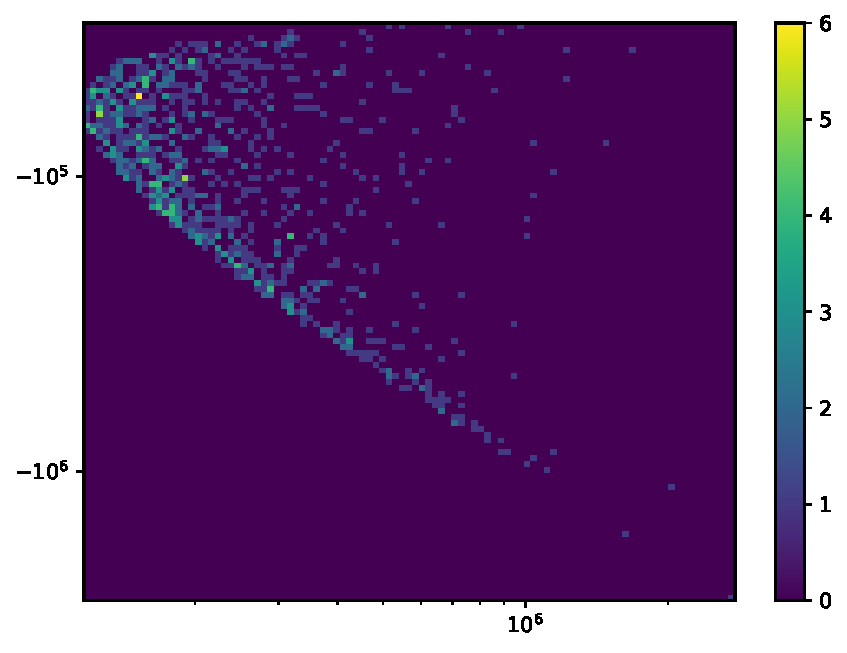
\includegraphics[width=0.25\textwidth]{plots/hardware_1k/ionQ/s-t_REAL_1000_100.pdf}%
  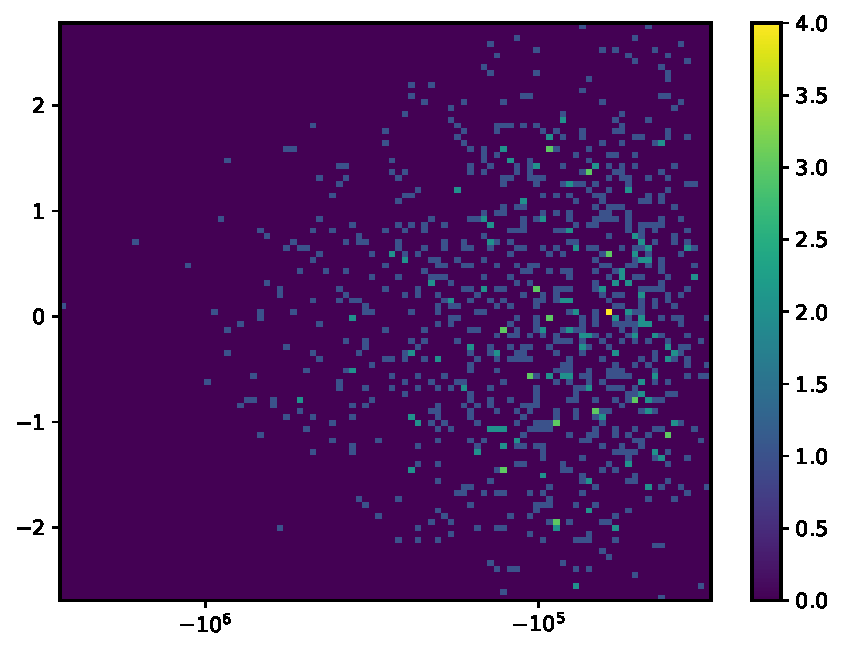
\includegraphics[width=0.25\textwidth]{plots/hardware_1k/ionQ/t-y_REAL_1000_100.pdf}%
  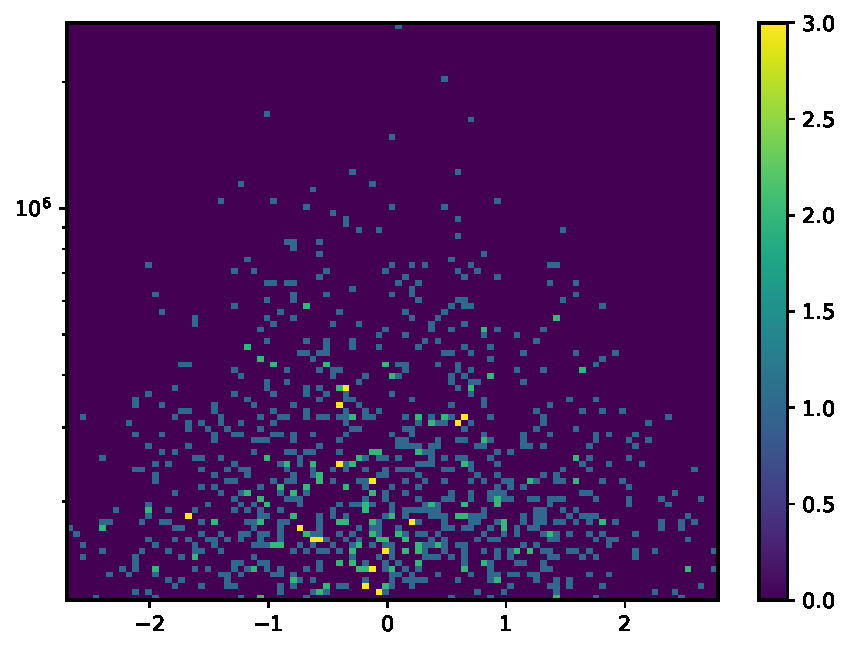
\includegraphics[width=0.25\textwidth]{plots/hardware_1k/ionQ/y-s_REAL_1000_100.pdf}

  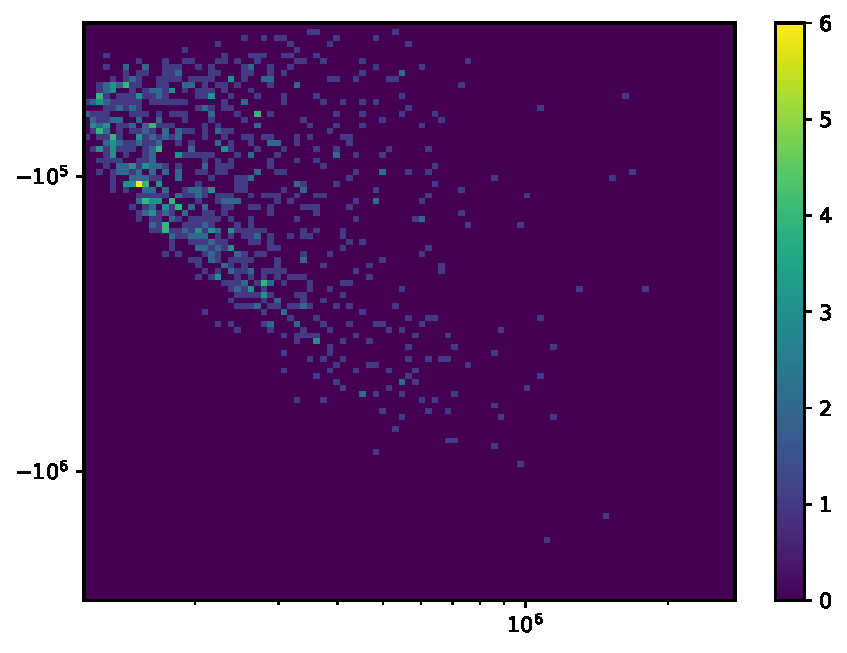
\includegraphics[width=0.25\textwidth]{plots/hardware_1k/ionQ/s-t_FAKE_1000_100_3_5_2_10000_128_0.5_1024.pdf}%
  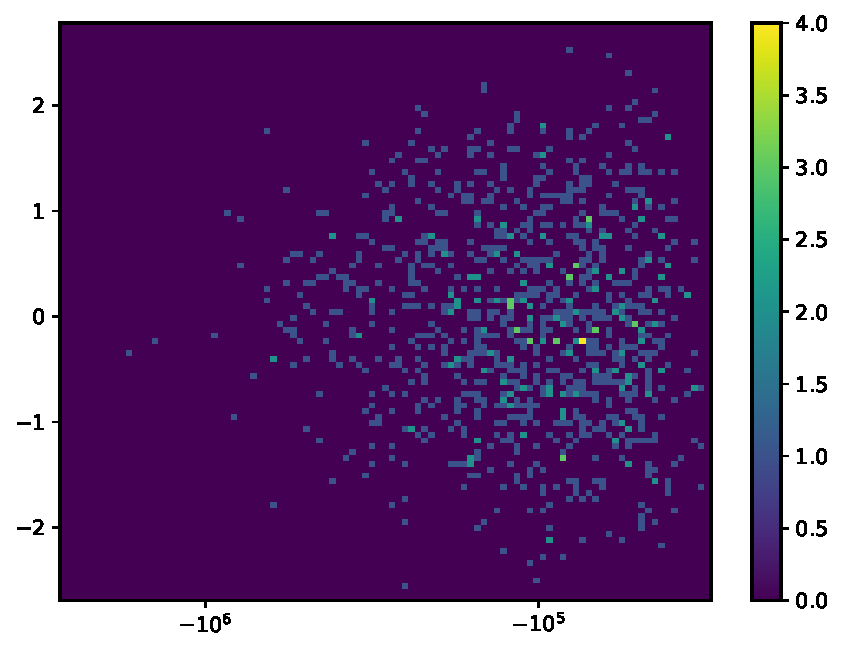
\includegraphics[width=0.25\textwidth]{plots/hardware_1k/ionQ/t-y_FAKE_1000_100_3_5_2_10000_128_0.5_1024.pdf}%
  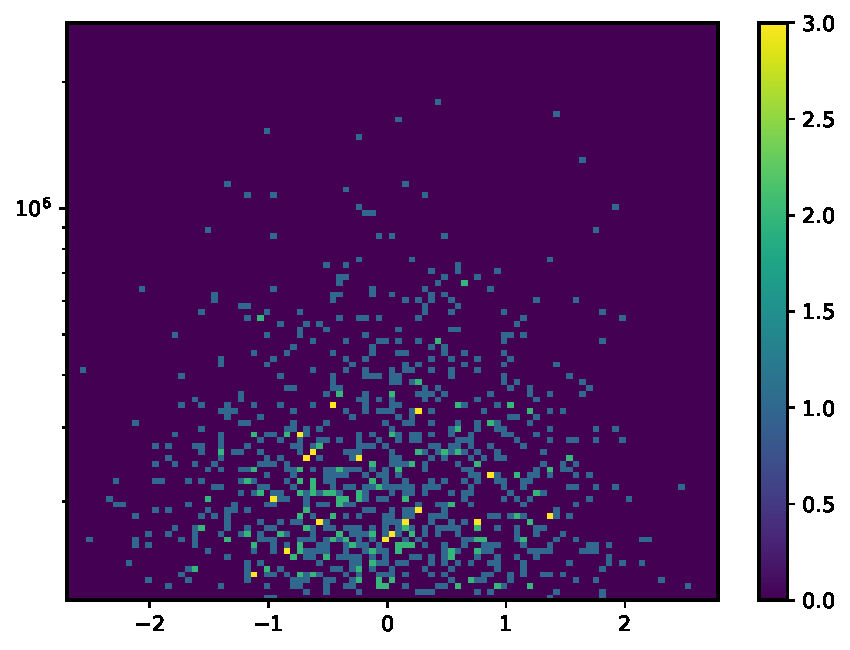
\includegraphics[width=0.25\textwidth]{plots/hardware_1k/ionQ/y-s_FAKE_1000_100_3_5_2_10000_128_0.5_1024.pdf}

  \caption{\label{fig:3dgauss}Example of samples generated for a $t\bar{t}$
  production using a QGAN generator model on IonQ.}
\end{figure*}


\section{Correlation analysis}

{\color{red}[SC: Anthony please summarize your results]}

\section{Conclusion}
\label{sec:conclusion}

In this work we proposed variational quantum circuit models for the generation
of Monte Carlo events in the context of high energy physics (HEP). We have
investigated and identified the most suitable Ansatz for the parametrization of
a quantum generative network. Using quantum circuit simulation on classical
hardware, we show that qMCGAN generators are suitable for Monte Carlo event
simulation.

We highlight some advantages of the qMCGAN model when compared to the standard
machine learning methodology. From a hardware implementation point of view, the
possibility to write the specific qMCGAN circuit in a quantum processor, using
its primitives (gates), will accelerate the evaluations and training performance
of Monte Carlo sampling. We expect that real quantum devices will be more
efficient in terms of energy power than classical hardware based on hardware
accelerators such as graphical process units (GPUs).

Furthermore, we propose a reconstruction method for evaluating the qMCGAN model
in a real quantum device using measurements. This procedure brings all the
difficulties that are typical of experimental quantum hardware, including noise,
error corrections and decoherence. The implementation of accurate and stable
qMCGAN in a real quantum device still requires the development of hardware
architecture with lower gate error tolerances in comparison to the current
available machines.

On the other hand, our results should be considered as a proof-of-concept
exercise, given that the quantum simulation performance are still not
competitive with an equivalent machine learning implementation. The qMCGAN
approach may show advantages when more precise quantum devices will be
available.

Nevertheless, this is a first attempt to bridge the power of quantum machine
learning algorithms into the complexity of Monte Carlo simulation in HEP. We
auspicate that the approach presented here will inspire new HEP applications
which may benefit from quantum computing.

\acknowledgments

This project is supported by CERN's QTI. SC is supported by the European
Research Council under the European Union's Horizon 2020 research and innovation
Programme (grant agreement number 740006).

\bibliography{qgan.bib}

\end{document}
